\documentclass[11pt]{article}

\usepackage{fullpage}
\usepackage{amsfonts}
\usepackage{graphicx}


\def\eq1{y=\frac{x}{3x^2+x+1}}
\def\labelaxes{Remember to include a scale and label your axes.}

\begin{document}

\begin{center}
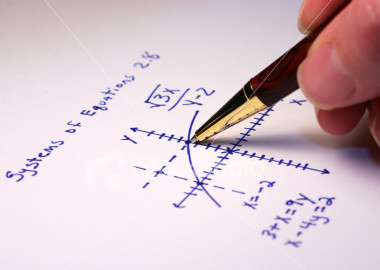
\includegraphics[angle=45]{algebra.jpg}

Images must be saved as .png, .jpg, .gif, or .pdf files.
\end{center}

The set of Natural numbers is denoted by $\mathbb{N}$.

The set of Integers is denoted by $\mathbb{Z}$.

The set of Real numbers is denoted by $\mathbb{R}$.

Graph $\eq1$. \labelaxes

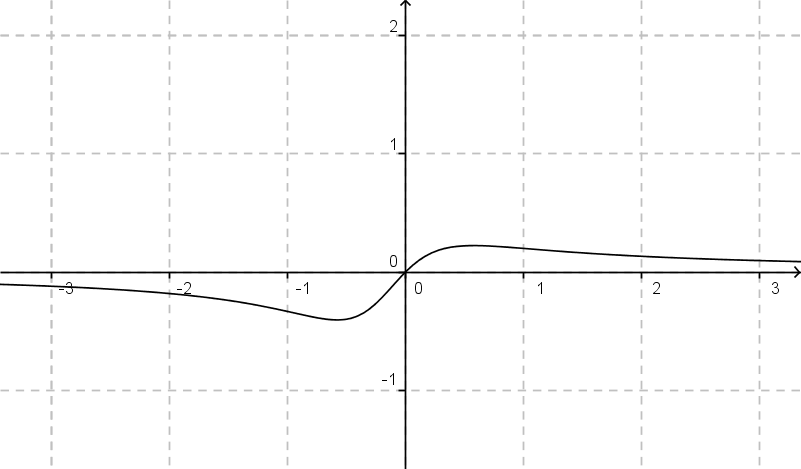
\includegraphics[width=5in]{quad1.png}

Identify the asymptotes for the graph of $\eq1$.

\end{document}